\begin{frame}{\insertsubsection}

  \begin{columns}
    \begin{column}{0.6\textwidth}
    Memory corruption
    \begin{itemize}
    \item Using uninitialized memory
    \item Using non-owned memory (null pointer, dangling pointer dereference,
      out of bounds error)
    \item Using memory beyond the memory that was allocated (buffer overflow)
    \item Faulty heap memory management (memory leaks, freeing non-heap or
      un-allocated memory)
    \end{itemize}
  \end{column}
  \begin{column}{0.4\textwidth}
    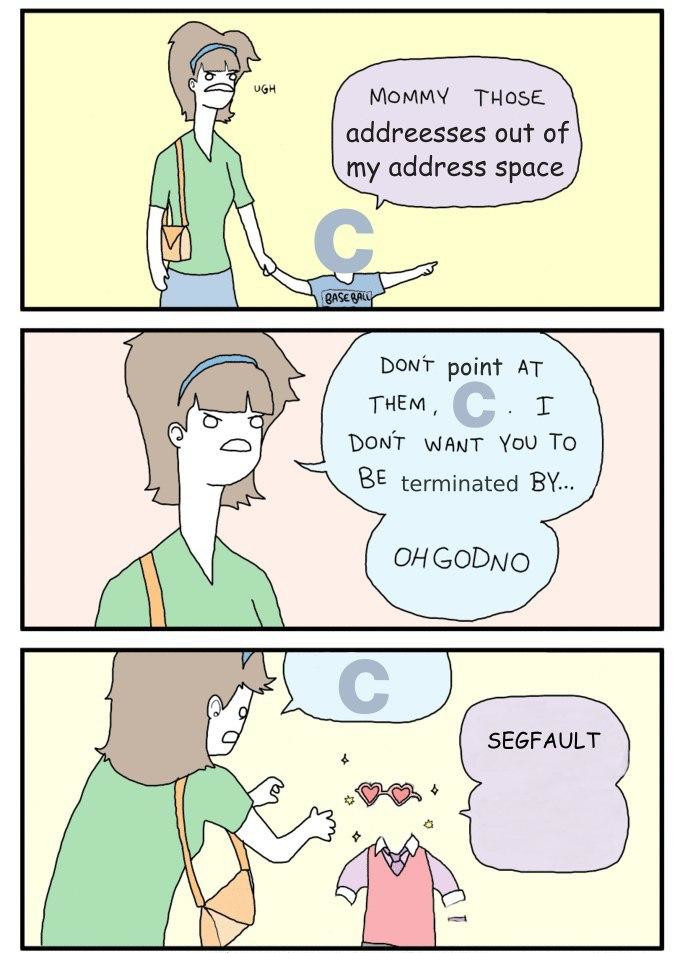
\includegraphics[width = 0.8\textwidth]{c_out_of_space.jpg}
  \end{column}
\end{columns}

  \note{

    В системных (и не только: Java, C\#) языках \textbf{существуют проблемы с
      безопасностью при работе с памятью}. Rust нацелен на решение этих самых
    проблем.

    Примеры проблем:

    \begin{itemize}
    \item использование не инициализированной памяти;
    \item использование не принадлежащей программе памяти;
    \item использование памяти за пределами выделенной;
    \item ошибки управления памятью на куче.
    \end{itemize}
    
  }
\end{frame}
